\section{Encoder}
The Encoder has the task of compressing the high-dimensional input data into a compact and manageable representation. It is a component of the Variational Auto-Encoder architecture, enabling the compression of input to latent variables.
The encoded data should capture important characteristics and features from the input data necessary for decompression while also removing unessesary and reduntant information. 
It operates by using a block like structure, where each block is designed to process the input data sequentially.

\subsection{Downsampling blocks}
Downsampling blocks are integral components within encoder architectures, facilitating the reduction of dimensionality of the feature maps. Based on the principles of CNNs the downsampling is achieved through a convolutional layer, that not only detects patterns within the input data but also strategically reduces the dimensions of the input.
The convolutional layer applies filters to the input, creating activation maps that highlight significant features. By adjusting the stride of the convolution, the layer can downsample the input, distilling the information into a more compact form. 

Following the convolutional layer, batch normalization is employed. This technique normalizes the output of the convolution by adjusting and scaling the activations. It allows the network to use higher learning rates, as it reduces the internal covariate shift which in turn makes the learning process more efficient and stable, as described by Ioffe and Szegedy\cite{batchnorm}.

\subsection{Residual block}
To enhance the encoder's ability to learn complex patterns and facilitate the training of deeper networks, residual blocks are integrated. These blocks, which were first introduced by He et al. in their paper on deep residual learning \cite{ResLearn}, incorporate shortcut connections that bypass one or more layers. 
The primary advantage of these shortcuts is to allow gradients to flow directly through the network, mitigating the vanishing gradient problem that often plagues deep neural networks. 

\begin{figure}[H]
    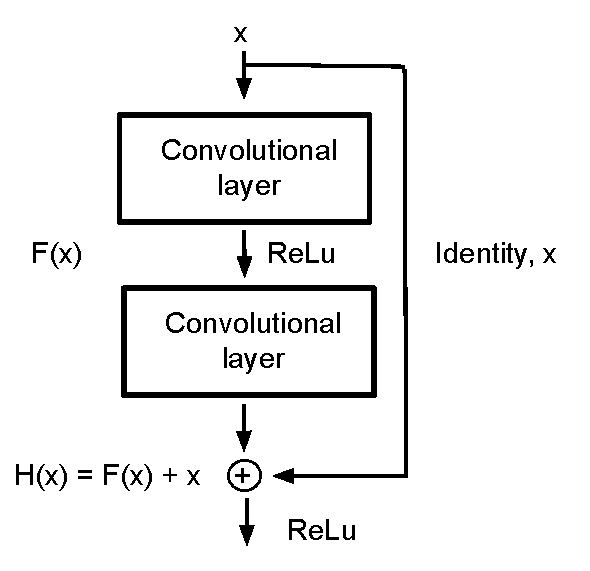
\includegraphics[scale=0.6]{figures/figure-pdf/Resnet.pdf}
    \caption{Illustration of the Resnet block from He et al's original paper\cite{ResLearn} }
\end{figure}


\subsection{Encoder Architecture}
The complete encoder architecture comprises a sequence of downsampling blocks, each further distilling the data. This is then followed by a series of Residual blocks to form deeper representations efficiently. The overall structure is sequential, with each block building upon the previous one to gradually reduce the input data's dimensionality while capturing
patterns and important features. The number of downsampling blocks is determined by a downsampling rate which is dependent of the size of the input data, and the amount of compression needed for the encoding task.

\begin{figure}[H]
    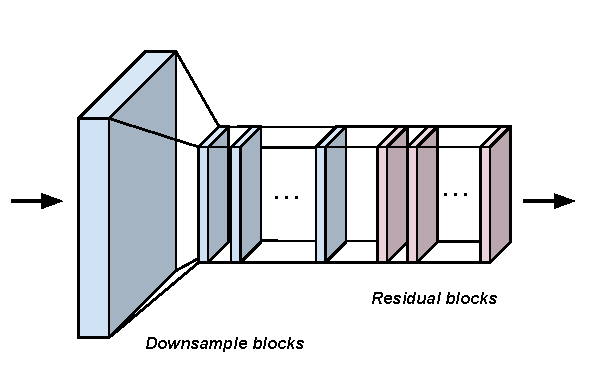
\includegraphics[scale=0.8]{figures/figure-pdf/Encoder.pdf}
    \caption{Illustration of the Encoder architecture used in the VQVAE implementation. The first downsample block reduces the dimensionality, followed by further downsample blocks to capture important features.}
\end{figure}

\section{Decoder}
While the encoder is responsible for data compression, the decoder is responsible for decompression. Instead of reducing the dimensions of the data, it will upsample it to a higher dimensional space.

\subsection{Upsampling Blocks}
Contrary to the encoder's downsampling blocks, the decoder employs upsampling blocks designed to incrementally reconstruct the higher-dimensional data from the lower-dimensional representation.  
The upsampling process is achieved through the use of transposed convolutional layers, often referred to as deconvolutional layers. These layers effectively reverse the operation of convolution by learning to expand a compressed feature map onto a larger spatial canvas.
The transposed convolutions apply filters in a manner that distributes the encoded feature values over a higher-resolution grid, interpolating additional data points as necessary to achieve the desired output size.
This process not only increases the spatial dimensions but also refines the feature map to recover details that were compressed during encoding.
Following the transpose convolutional layer the upsample block uses batch normalization and ReLu activation function.


\subsection{Decoder Architecture}
The decoder's architecture is characterized by a series residual blocks followed by upsampling blocks that progressively restore the data's dimensionality. The number of upsampling blocks is the same as number of downsampling blocks in the encoder. 
